\subsection{Logical Operations \& Bit Masking}

\begin{lstlisting}
B7: EQU $80 ; Mask for Bit 7
B6: EQU $40 ; Mask for Bit 6
 :     :           :
B0: EQU $01 ; Mask for Bit 0

ORA #(B6 | B3) ; Set Bit 6 and 3 in ACCU
AND #(B5 | B4) ; Delete all Bits in ACCU except Bit 5 and 4
\end{lstlisting}

\begin{tabular}{lp{0.3\textwidth}}
    \textbf{AND} & \textit{logical AND-operation} \\
    \textbf{ORA} & \textit{logical OR-operation} \\
    \textbf{EOR} & \textit{logical XOR-operation} \\
    \textbf{BCLR n,Addr} & \textit{Delete Bit n on a specific memory address} \\
    \textbf{BSET n,Addr} & \textit{Set Bit n on a specific memory address} \\
    \textbf{BIT Addr} & \textit{
        Bitwise AND operation of Accu with content of Addr,
        without changing content of Accu and Addr.
        Affects only \textbf{N- and Z-Flags}.
    } \\
    \textbf{CLC} & \textit{Delete \textbf{Carry}-Flag C} \\
    \textbf{SEC} & \textit{Set Carry-Flag C} \\
    \textbf{CLI} & \textit{Delete \textbf{Interrupt}-Mask Bit I (Interrupt \textbf{enable})} \\
    \textbf{SEI} & \textit{Set Interrupt-Mask Bit I (Interrupt disable)} \\
\end{tabular}

\subsection{Shift- and Rotation Operations}

\begin{tabular}{ll}
    \textbf{in direction MSB (left)} & \textbf{in direction LSB (rigth)} \\
    \\
    Logical Operations: \\
    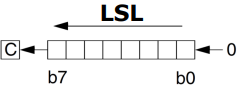
\includegraphics[width=0.24\textwidth]{operand-lsl.png} &
    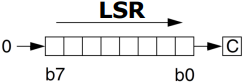
\includegraphics[width=0.24\textwidth]{operand-lsr.png} \\
    \\
    Arithmetic Operations: \\
    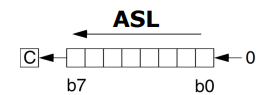
\includegraphics[width=0.24\textwidth]{operand-asl.png} &
    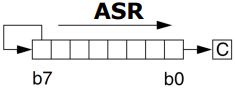
\includegraphics[width=0.24\textwidth]{operand-asr.png} \\
    \textit{Multiplication by 2, ASL=LSL} &
    \textit{Division by 2} \\
    \\
    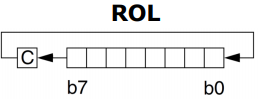
\includegraphics[width=0.24\textwidth]{operand-rol.png} &
    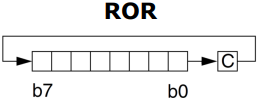
\includegraphics[width=0.24\textwidth]{operand-ror.png} \\
\end{tabular}

\subsection{Relative Branching}

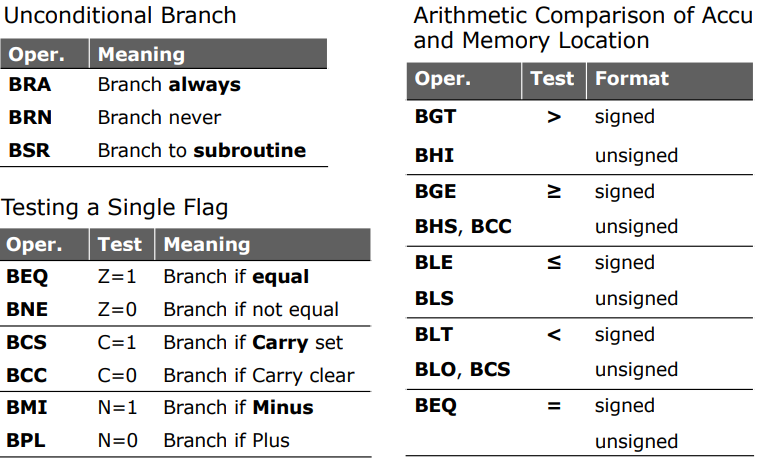
\includegraphics[width=0.5\textwidth]{operation-branching.png}

\subsection{Branching Compare-Operation}

\textit{
    Compare instructions are \textbf{subtraction operations} that change status
    flags, but leave the data registers unchanged.
}

\begin{tabular}{rp{0.35\textwidth}}
    \textbf{CMP opr8} & \textit{Compare content of \textbf{ACCU} with 8-bit operand} \\
    \textbf{CPX opr8} & \textit{Compare content of \textbf{X-Register} with 8-bit operand} \\
    \textbf{CMP opr8} & \textit{Compare content of \textbf{HX-Register} with 16-bit operand} \\
\end{tabular}

\textit{
    Example, Test if a value is bigger or smaller than
    another value, branch afterwards
}

\begin{lstlisting}
LDA Op1
CMP Op2   ; Calculates (Op1-Op2) and sets flags
BMI Label ; Branch if Op2 > Op1 (N=1) to Label
\end{lstlisting}

\subsection{Direct relative Branching}

\textit{
    Those Branches are dependent on a single Bit of a memory located
    in the \textbf{Direct Page}.
}

\begin{lstlisting}
BRCLR n,Addr,Label ; Branches to Label, if Bit n of value on
                   ;address Addr is not set (Addr only DIR)
BRSET n,Addr,Label ; Branches to Label, if Bit n of value on
                   ;address Addr is set (Addr only DIR)
\end{lstlisting}
